%!TeX root = ./00.ppgcc-2020.tex

\section{Implementação com MPI}

Com os desafios de distribuição e memória encontrados nas implementações
preliminares, optou-se por tomar mais controle sobre estes aspectos para
maximizar o aproveitamento do \emph{hardware} escolhido visto que seus recursos
são limitados.
Para isso escolheu-se implementar a proposta utilizando a \acf{MPI} e linguagem C,
onde tem-se controle fino sobre o uso de memória e distribuição, no entanto
perde-se a perícia incluída nas plataformas tradicionais que oferecem
facilidades e garantias necessárias em contextos de ``produção''
(\emph{software} em execução em um ambiente corporativo, que garante o
funcionamento confiável e contínuo de uma corporação).

O algoritmo \minas original \cite{Faria2016minas} tem uma implementação
companheira\footnote{Disponível em \url{http://www.facom.ufu.br/~elaine/MINAS}}
\cite{Faria2013source}, aqui referida como \refminas, escrita em Java utilizando
os algoritmos base como \emph{K-means} e \emph{CluStream} da biblioteca MOA
\cite{MOA}.
Esta implementação serve de referência para a construção provendo validação dos
resultados e servindo também de comparação básica de desempenho.

Os primeiros pontos de divergência do \mfog e \refminas são o algoritmo de
agrupamento e cálculo de raio.
Enquanto \refminas permite a escolha entre \emph{K-means} e \emph{CluStream} para a
fase \emph{offline} e \emph{online}, \mfog implementa apenas \emph{K-means}.
O cálculo de raio em \refminas é definido com o máximo do conjunto de distância
dos exemplos de um \mcluster ao seu centro, seguindo a Equação \ref{eq:raio_max},
enquanto o \mfog segue a definição em \citeonline{Faria2016minas} utilizando o
desvio padrão dos valores do mesmo conjunto de distâncias multiplicado pelo
parâmetro $f_{raio}$ seguindo a Equação \ref{eq:raio_paper}.

\newcommand{\val}{$\vec{v}\,$\xspace}
Os formatos dos fluxos de dados de entrada e de saída também são notáveis. Como
entrada, o algoritmo da proposta recebe dois fluxos, o principal é o que contém
os exemplos, sendo cada exemplo um vetor de números de dimensão $d$.
O segundo fluxo de entrada consiste de \mclusters representando o modelo inicial
criado e capturado da fase de treinamento \emph{offline}.
A fase de treinamento \emph{offline} foi implementada mas não sofre alteração
com relação ao algoritmo \minas \cite{Faria2016minas} além da execução separada
com conjunto de treinamento similar à definição do fluxo de exemplos principal
com adição de uma dimensão com valor de um caractere marcando a classe conhecida
e saída como um fluxo finito de \mclusters.

O formato do fluxo de saída é definido como a tripla contendo o número de
sequência do exemplo no fluxo de entrada (\emph{uid}), etiqueta de um caractere
atribuída ao exemplo e tempo em milissegundos entre a ingestão (entrada) e saída
do exemplo no sistema.

% - Reprocessamento dos exemplos utilizados para atualização do modelo:
%   - Muda o comportamento do operador de fluxo de `Map` para `Flatmap`, ou seja,
%     requer outro fluxo de saída para a transmissão de padrões novidade (alarmes);
%   - Para reclassificação a definição de raio é modificada de `r = f * σ` (fator
%     multiplicando desvio padrão) para `r = max(distance)` (distância máxima);
%   - Passível da crítica de *overfitting*. Isto é, este processo pode
%     inflar a métrica de precisão;
%   - **Solução:** *em aberto*;


\begin{algorithm}[htb]
    % {\scriptsize
    % \begin{multicols}{2}
    % \SetAlgoVlined
    \SetKwProg{Function}{Function}{:}{}
    \SetKwFor{With}{with}{}{}
    \SetKw{continue}{continue}
    % 
    \SetKwData{MEPC}{MEPC}
    \SetKwData{NF}{NF}
    \SetKwData{mpiSize}{mpiSize}
    \SetKwData{mpiRank}{mpiRank}
    \SetKwData{EndOfStream}{EndOfStream}
    % 
    \SetKwInOut{KwParams}{Parameters}
    \KwParams{mpiNodeRank as \mpiRank}
    % 
    \SetKwFunction{Mfog}{Mfog}
    \SetKwFunction{Sampler}{Sampler}
    \SetKwFunction{Classifier}{Classifier}
    \SetKwFunction{Detector}{Detector}
    \SetKwFunction{modelReceiver}{modelReceiver}
    % 
    \SetKwFunction{typeOf}{typeOf}
    % 
    \SetKwFunction{Thread}{Thread}
    \SetKwFunction{Lock}{Lock}
    \SetKwFunction{readLock}{readLock}
    \SetKwFunction{writeLock}{writeLock}
    % 
    \SetKwFunction{receive}{receive}
    \SetKwFunction{send}{send}
    \SetKwFunction{broadcast}{broadcast}
    % 
    \SetKwFunction{nearestCluster}{nearestCluster}
    \SetKwFunction{NoveltyDetection}{NoveltyDetection}
    \SetKwFunction{handleModelSleep}{handleModelSleep}
    \SetKwFunction{removeOldSamples}{removeOldSamples}
    \SetKwFunction{now}{now}
    % 
    \KwIn{ModelSet, Sample Stream}
    % \KwOut{Classified Stream as $out$}
    % 
    \Function{\Mfog{ModelStream, InputStream, OutputStream}}{
        ModelSet = $\emptyset$\;
        ModelSetLock = \textbf{new} \Lock()\;
        \eIf(\emph{root}){\mpiRank == 0}{
            \textbf{new} \Thread(\Detector, [OutputStream, ModelSet, ModelSetLock])\;
            \Sampler(InputStream, ModelSet, ModelSetLock)\;
        }(\emph{leaf}){
            \textbf{new} \Thread(\modelReceiver, [ModelSet, ModelSetLock])\;
            \Classifier(ModelSet, ModelSetLock)\;
        }
    }
\caption{MFOG: main MPI entry-point.}
\label{alg:MFOG}
\end{algorithm}

\begin{algorithm}[htb]
    \SetKwFor{With}{with}{}{}
    \SetKw{continue}{continue}
    % 
    \SetKwData{MEPC}{MEPC}
    \SetKwData{NF}{NF}
    \SetKwData{mpiSize}{mpiSize}
    \SetKwData{mpiRank}{mpiRank}
    \SetKwData{EndOfStream}{EndOfStream}
    % 
    \SetKwProg{Function}{Function}{:}{}
    \Function{\Classifier{ModelSet, ModelSetLock}}{
        \While{ True }{
            sampe = \receive(SampleType, root)\;
            \lIf{sample == \EndOfStream}{\textbf{break}}
            sample.label = unknown\;
            \With{\readLock(ModelSetLock)}{
                (distance, cluster) = \nearestCluster(sample, ModelSet)\;
            }
            \If{distance $<$ cluster.radius}{
                sample.label = cluster.label\;
            }
            \send(root, SampleType, sample)\;
        }
    }
    %     \label{alg:MFOG-classifier}
    %     \caption{MFOG: Classifier task.}
    % \end{algorithm}
    % \begin{algorithm}
    % \SetKwProg{algorithm}{algorithm}{:}{}
    \SetKwFor{With}{with}{}{}
    \SetKw{continue}{continue}
    % 
    \SetKwData{MEPC}{MEPC}
    \SetKwData{NF}{NF}
    \SetKwData{mpiSize}{mpiSize}
    \SetKwData{mpiRank}{mpiRank}
    \SetKwData{EndOfStream}{EndOfStream}
    % 
    \SetKwProg{Function}{Function}{:}{}
    \Function{\modelReceiver{ModelSet, ModelSetLock}}{
        \While{ True }{
            cl = \receive(ClusterType, root)\;
            \lIf{cl == \EndOfStream}{\textbf{break}}
            \With{writeLock(ModelSetLock)}{
                ModelSet = ModelSet $\cup$ cl\;
            }
        }
    }
    % \label{alg:MFOG-model}
    % \caption{MFOG: model receiver task.}
\caption{MFOG Leaf Tasks: Model Receiver and Classifier.}
\label{alg:MFOG-leaf}
\end{algorithm}
\begin{algorithm}[htb]
    \SetKwFor{With}{with}{}{}
    \SetKw{continue}{continue}
    % 
    \SetKwData{MEPC}{MEPC}
    \SetKwData{NF}{NF}
    \SetKwData{mpiSize}{mpiSize}
    \SetKwData{mpiRank}{mpiRank}
    \SetKwData{EndOfStream}{EndOfStream}
    \SetKwInOut{KwParams}{Parameters}
    \KwParams{mpiClusterSize as \mpiSize}
    \SetKwProg{Function}{Function}{:}{}
    \Function{\Sampler{InputStream, ModelSet, ModelSetLock}}{
        % ModelSet = read()\;
        % broadcast(ModelSet)\;
        dest = 1\;
        \ForEach{ sample from InputStream }{
            \If{\typeOf(sample) is Cluster}{
                \broadcast(ClusterType, sample, root)\;
                \With{\writeLock(ModelSetLock)}{
                    ModelSet = ModelSet $\cup$ sample\;
                }
                \continue\;
            }
            % sample.label = unknown\;
            \send(dest, SampleType, sample)\;
            dest = dest $+ 1$\;
            \lIf{dest $>$ \mpiSize}{dest = 1}
        }
    }

    %     \label{alg:MFOG-sampler}
    %     \caption{MFOG: sampler Module.}
    % \end{algorithm}
    % \begin{algorithm}
    \SetKwProg{algorithm}{algorithm}{:}{}
    \SetKwFor{With}{with}{}{}
    \SetKw{continue}{continue}
    % 
    \SetKwData{cleaningWindow}{cleaningWindow}
    \SetKwFunction{removeOldSamples}{removeOldSamples}
    \SetKwData{noveltyDetectionTrigger}{noveltyDetectionTrigger}
    \SetKwData{MEPC}{MEPC}
    \SetKwData{NF}{NF}
    \SetKwData{mpiSize}{mpiSize}
    \SetKwData{mpiRank}{mpiRank}
    \SetKwData{EndOfStream}{EndOfStream}

    \KwParams{\cleaningWindow, \noveltyDetectionTrigger}

    \SetKwProg{Function}{Function}{:}{}
    \Function{\Detector{OutputStream, ModelSet, ModelSetLock}}{
        lastCleanup $\leftarrow 0$\;
        \While{ True }{
            sampe = \receive(SampleType, any)\;
            \lIf{sample == \EndOfStream}{\textbf{break}}
            % $out \leftarrow$ sample\;
            OutputStream.append(sample)\;
            \If{sample.label == unknown}{
                UnknownSet = UnknownSet $\cup$ sample\;
                \If{$|\;UnknownSet\;| \geq$ \noveltyDetectionTrigger}{
                    novelties = \NoveltyDetection(ModelSet, *UnknownSet)\;
                    \With{\writeLock(ModelSetLock)}{
                        ModelSet = ModelSet $\cup$ novelties\;
                    }
                    \ForEach{ cl in novelties }{
                        \broadcast(ClusterType, cl, root)\;
                    }
                }
                \If{ sampe.uid $ > $ ( lastCleanup $ + $ \cleaningWindow )}{
                    UnknownSet $\leftarrow$ \removeOldSamples(UnknownSet, lastCleanup)\;
                    lastCleanup $ \leftarrow $ sampe.uid\;
                }
            }
        }
    }
    % \label{alg:MFOG-detector}
    % \caption{MFOG: detector task.}
\caption{MFOG Root Tasks: Sampler and Detector.}
\label{alg:MFOG-root}
\end{algorithm}

For evaluation purposes, an \mfog implementation was made using MPI (\emph{Open
MPI 4.0.4}).
The program is organized in a single program multiple data (SPMD)
programming model, so a single version of the \mfog program was initiated on all
nodes, being that one of them would perform the root role, while the others ran
as leaves, the program entry point is illustrated on Algorithm \ref{alg:MFOG}.
On the root process, a sampler thread is responsible for distributing the
sampled flow information (\val) to the classifier nodes, using a round-robin
load balancing scheme.
The other thread on the root process is responsible for receiving the
classification results and for processing the unknown samples in the search for
novelties.
The root process functions are illustrated in Algorithm \ref{alg:MFOG-root}.
Each leaf node runs a model adjustment thread and multiple (up to the number of
cores) classifier threads. The leaf tasks are illustrated in Algorithm
\ref{alg:MFOG-leaf}.
The overall sequence of interactions is shown in Figure \ref{fig:mfog-mpi-life}.

\begin{figure}[htb]
  \centerline{
    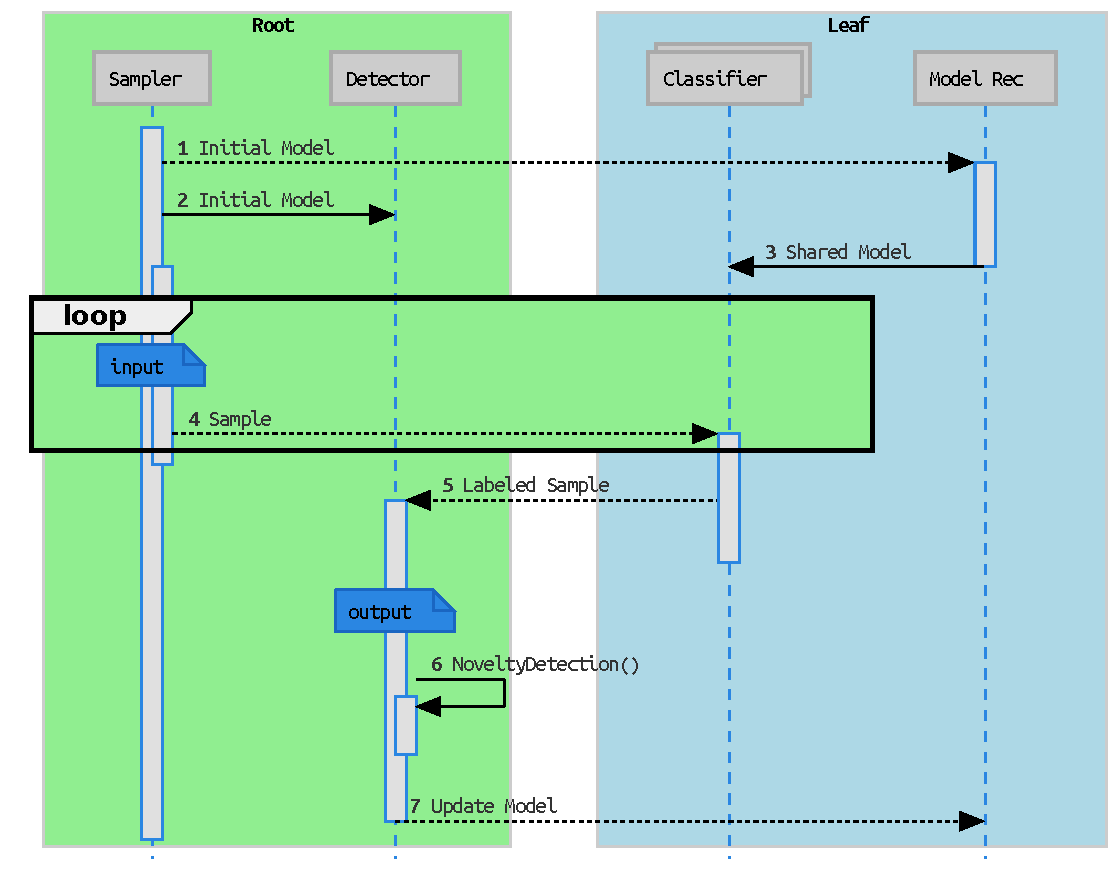
\includegraphics[width=0.75\linewidth,page=1]{figures/lifecycle-uml-svg.pdf}
  }
  \caption{\mfog life line overview.}
  \label{fig:mfog-mpi-life}
\end{figure}
